
% @author Jan Robert Rösler 
%
\chapter{Neuronale Navigation mit Bilddaten}

\section{Relevante Technik/Hintergrund}
Hier erfolgt zunächst eine kurze Beschreibung der für Neuronale Navigation auf Bilddaten relevanten Technik. Grundlegendes wird nur der Vollständigkeit halber erwähnt, speziellere Aspekte kurz vorgestellt. 

\subsection{Deep Learning}

\subsection{CNN}
\textit{Convolutional Neural Networks}, oder kurz CNN, haben sich gerade im Bereich der Bildverarbeitung als überlegen bewiesen. Aus der Biologie inspiriert, findet hier besonders das Prinzip des rezeptiven Feldes Anwendung. Die Aktivität jedes Neurons wird mithilfe einer Faltung berechnet, räumliche Informationen und Zusammenhänge werden so besser erhalten. 2012 konnte ein CNN, AlexNet \cite{krizhevsky2012imagenet}, beim ImageNet-Wettbewerb den Benchmark-Rekord von 25,8 \% auf 16,4 \% drücken, seitdem sind alle gut platzierten Modelle CNNs.
CNNs sollen hier nicht detailliert erklärt werden, das Verständnis wird als Grundlage vorausgesetzt.

\subsection{ResNet}
\textit{Residual Neural Networks}, oder kurz ResNet, ist eine weitere Technik, die ihren Urprung in der Biologie hat. Verhalten so genannter Pyramidenzellen, Nervenzellen im menschlichen Gehirn, wird nachgebildet, indem Abkürzungen zwischen Layer eingebaut werden. Residual Netze wurden 2015 entwickelt, insbesondere ließ sich mit diesem Ansatz das trainieren tiefer Netze verbessern \cite{DBLP:journals/corr/HeZRS15}. \ref{img:ResBlock} zeigt den schematischen Aufbau eines so genannten Residual Blocks. 


\begin{figure}
	\centering
	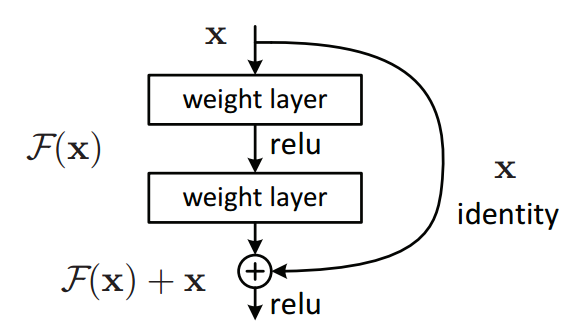
\includegraphics[scale=0.5]{figures/ResidualBlock.png}
	\caption{Residual Block}
	Quelle: \citeI{ResBlock}
	\label{img:ResBlock}
\end{figure}


DBLP:journals/corr/HeZRS15

\subsection{Fine tuning}
LAYER FREEZING 
Fine Tuning 









\section{Ansätze}
Im folgenden wird auf zwei Ansätze der Navigation mit Neuronalen Netzen eingegangen, durch Gegenüberstellung erster Versuche mit einem modernen Ansatz soll folgenden Ausarbeitungen ein Rahmen gegeben werden.

\subsection{ALVINN}

Versuche durch neuronale Verarbeitung von reinen Bilddaten in einem Szenario zu navigieren, gab es bereits 1989 in Pomerleau's Arbeit, die man auf diesem Gebiet als Pionierarbeit verstehen kann.\cite{pomerleau1989alvinn}.
Das Netzwerk ALVINN (Autonomous Land Vehicle In a Neural Network) sollte das NAVLAB steuern, ein Testfahrzeug für Autonome Navigation der Carnegie Mellon University.
In \ref{img:ALVINNa} lässt sich die Architektur nachvollziehen. 
Der rein visuelle Input (die Blautstufenintensität eines Pixels bestimmt das Aktivierungslevel des Inputneurons) wird untersützt durch eine laserbasierte Abstandsmessung und ein Inputneuron für die Kodierung der \glqq Straßenintensität\grqq{}, also ob die Straße heller oder dunkler wird.
Aus heutiger Sicht ist das Netz mit nur einer hidden Layer mit 29 Neronen sehr klein, die im weiteren angesprochenen Architekturen haben deutlich mehr Layer und mehrere Hunderttausend Parameter. 
Zudem interpretiert ALVINN die Aufgabe des Spurfolgens nicht als Regressionsproblem, sondern als Klassifikation. Die Ausgangsneuronen sind eine lineare Repräsentation der Lenkrichtung, die das Fahrzeug in Richtung Fahrbahnmitte steuert. Neuronen in der Mitte stehen für eine Fahrt geradeaus, Neuronen links und rechts für die jeweilige Fahrtrichtung.
Grob gesagt gibt das Neuron mit dem höchsten Aktivierungslevel die Fahrtrichtung (den einzuschlagenden Lenkwinkel) an.
Im Ergebnis konnte das Netz nach 40 Epochen Training auf simulierten Fahrbahnbildern, zu sehen in \ref{img:ALVINNb}, einen 400 Meter Weg durch einen Wald mit \SI{1/2}{\meter/\second} sicher abfahren.//

\begin{figure}
	\centering
	\begin{subfigure}{.5\textwidth}
	\centering
		  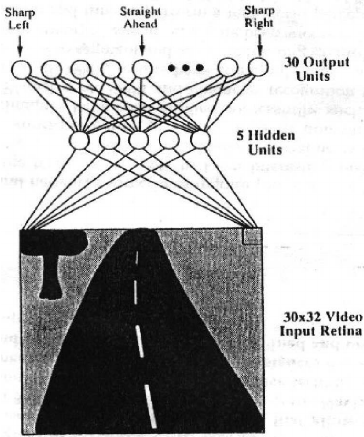
\includegraphics[width=.85\linewidth]{figures/Architecture-ALVINN.png}
		  \caption{}
		  \label{img:ALVINNa}
	\end{subfigure}%
	\begin{subfigure}{.5\textwidth}
	\centering
		  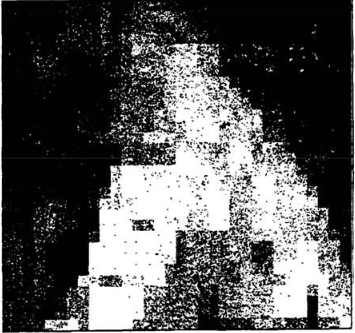
\includegraphics[width=.85\linewidth]{figures/Strasse-ALVINN.png}
	 	  \caption{}
		  \label{img:ALVINNb}
	\end{subfigure}%
	\caption{ALVINN Architektur (a) und simulierte Fahrbahn (b)}
	%Quelle: \protect\citeI{Architecture-ALVINN}
	\label{img:ALVINN}
\end{figure}

\subsection{NVIDIA DAVE-2}

Forschungserkenntnisse der folgenden Jahre trieben die Entwicklung voran und...
Im Jahr 2016 veröffentlicht das Technologieunternehmen \textsc{NVIDIA} einen eigenen Ansatz \cite{bojarski2016end}, basierend auf Versuchen mit dem \glqq DARPA Autonomous Vehicle \grqq{} (DAVE) \citeI{DarpaDave} wird dieser \glqq Dave-2 \grqq{} genannt.//
Daten werden hier durch Fahrten auf echten Straßen gesammelt, wofür drei Kameras in der Windschutzscheibe eines Autos angebracht wird und Steuerungsdaten über den CAN bus des Fahrzeuges ausgelesen werden. Mit diesen Daten wird ein CNN trainiert \ref{img:NVIDIA}, was dann an einer Straßen-Simulation getestet wird. Hervorzuheben ist hier besonders die Verwendung von Convolutional Neural Networks (CNN) und die, im Gegensatz zum bereits erwähnten Ansatz 27 Jahre zuvor, stark gesteigerte Rechenleistung. Folglich können nicht nur Bilder besserer Qualität verarbeitet werden, die Netzarchitektur mit 9 Layern und 250.00 Parametern wäre 1989 nicht in annehmbarer Zeit trainierbar gewesen. Außerdem stellt sich NVIDIA dem Anspruch, eine neuronale Steuerung für öffentliche Straßen zu entwerfen, nicht nur für ein sehr begrenztes Testszenario.



\begin{figure}
	\centering
	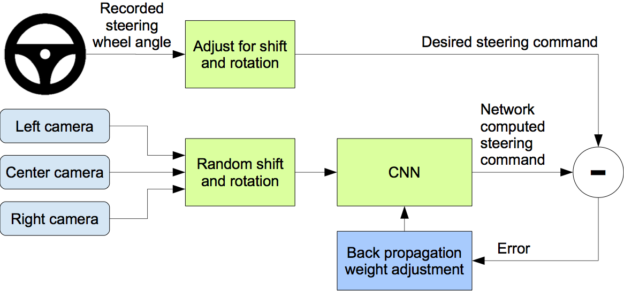
\includegraphics[scale=0.5]{figures/NVIDIA-Training.png}
	\caption{Komponenten des Trainings}
	Quelle: \citeI{NVIDIA-Components}
	\label{img:NVIDIA}
\end{figure}





 Präsentation ALVINN, dann gegenüberstellung mit modernem Netzwerk a la NVIDIA.






Kurzer Blick auf  Self driving car steering angle4 prediction und berkeley (large scale video sets) (vielleicht auchSPÄTER)




Glossar

Convolutional Neural Network CNN


